% !TeX root = ..\..\latex-talk.tex

\part{SJTUThesis}

\begin{frame}
  \frametitle{简介}
  \begin{columns}
    \begin{column}{0.6\textwidth}
      \begin{itemize}
        \item 最早由韦建文于 2009 年 11 月发布 0.1a 版,2018 年起由 SJTUG 接手维护
        \item 最新版:\SJTUThesisVersion{} (\SJTUThesisDate)
        \item 支持本科、硕士、博士学位论文以及课程论文的排版
      \end{itemize}
    \end{column}
    \begin{column}{0.4\textwidth}
      \begin{exampleblock}{}
        \begin{minipage}[c]{1cm}
          \includegraphics[width=0.8cm]{\getcontribpath{sjtug}{vi/sjtug}}
        \end{minipage}
        \begin{minipage}[c]{2cm}
          \href{https://github.com/sjtug}{sjtug}/\href{https://github.com/sjtug/SJTUThesis}{SJTUThesis}
        \end{minipage}
      \end{exampleblock}
      \vspace{-8pt}
      \begin{block}{}
        \scriptsize
        上海交通大学 \hologo{XeLaTeX} 学位论文及课程论文模板 | Shanghai Jiao Tong University \hologo{XeLaTeX} Thesis Template
      \end{block}
      \vspace{-8pt}
      \begin{alertblock}{}
        \scriptsize
        \begin{tabular}{cl}
          \faStar & 2.4k \\
          \faEye & 55 \\
          \faCodeBranch & 701 \\
        \end{tabular}
      \end{alertblock}
    \end{column}
  \end{columns}
\end{frame}

\begin{frame}
  \frametitle{下载与编译}
  \alert{下载} 推荐安装 Git \link{https://git-scm.com/} 后,克隆 SJTUG 镜像仓库
  \begin{exampleblock}{\faGit*}
    \ttfamily\small
    git clone https://mirror.sjtu.edu.cn/git/SJTUThesis.git/
  \end{exampleblock}

  \alert{编译} 推荐使用 \pkg{latexmk} 编译\footnote{\hologo{MiKTeX} 用户需要手动安装 Perl 解释器 \link{https://www.perl.org/get.html} 才能使用 \pkg{latexmk}。},在不能够利用自带的 \texttt{.latexmkrc} 配置文件的情况下,需要查清楚在对应的编辑器中如何使用 \hologo{XeLaTeX} + \hologo{biber} 编译 \link{https://github.com/sjtug/SJTUThesis/blob/master/README.md}。
  \begin{exampleblock}{\faTerminal}
    \ttfamily\small
    latexmk -xelatex main
  \end{exampleblock}

  Overleaf 用户可以下载压缩包后,上传并采用 \hologo{XeLaTeX} 编译方式。
\end{frame}

\begin{frame}[fragile, label=covers]
  \begin{codeblock}[firstnumber=3]{main.tex}
|\alert{\% 载入 SJTUThesis 模版}|
\documentclass[|\only<1>{\highlight{type}}\only<2>{type}|=|\only<1>{bachelor}\only<2>{\highlight{bachelor}}|]{sjtuthesis}
  \end{codeblock}
  \begin{figure}
    \parbox{0.9\textwidth}{
      \begin{subfigure}{0.20\textwidth}
        \framebox{\includegraphics[width=\linewidth]{support/thesis/bachelor}}
        \caption{\only<1>{学士}\only<2>{\texttt{bachelor}}}
      \end{subfigure}\hfill
      \begin{subfigure}{0.20\textwidth}
        \framebox{\includegraphics[width=\linewidth]{support/thesis/master}}
        \caption{\only<1>{硕士}\only<2>{\texttt{master}}}
      \end{subfigure}\hfill
      \begin{subfigure}{0.20\textwidth}
        \framebox{\includegraphics[width=\linewidth]{support/thesis/doctor}}
        \caption{\only<1>{博士}\only<2>{\texttt{doctor}}}
      \end{subfigure}\hfill
      \begin{subfigure}{0.20\textwidth}
        \framebox{\includegraphics[width=\linewidth]{support/thesis/course}}
        \caption{\only<1>{课程}\only<2>{\texttt{course}}}
      \end{subfigure}
      \caption{论文类型示例\only<2>{ \texttt{type}}}
    }
  \end{figure}
\end{frame}

\begin{frame}[fragile]
  \frametitle{基本配置}
  \framesubtitle{\texttt{\textbackslash{}input\{setup\}}}
  \begin{columns}
    \begin{column}{0.45\textwidth}
      \includegraphics[page=9]{thesisdir}
    \end{column}
    \begin{column}{0.55\textwidth}
      \begin{codeblock}[firstnumber=12]{main.tex}
|\highlightline<1>|% 论文基本配置,加载宏包等全局配置
|\highlightline<1>|% !TEX root = ./main.tex

\sjtusetup{
  %
  %******************************
  % 注意:
  %   1. 配置里面不要出现空行
  %   2. 不需要的配置信息可以删除
  %******************************
  %
  % 信息录入
  %
  info = {%
    %
    % 标题
    %
    title           = {上海交通大学学位论文 \LaTeX{} 模板示例文档},
    title*          = {A Sample Document for \LaTeX-based SJTU Thesis Template},
    %
    % 标题页标题
    %   可使用“\\”命令手动控制换行
    %
    % display-title   = {上海交通大学学位论文\\ \LaTeX{} 模板示例文档},
    % display-title*  = {A Sample Document \\ for \LaTeX-based SJTU Thesis Template},
    %
    % 页眉标题
    %
    % running-title   = {示例文档},
    % running-title*  = {Sample Document},
    %
    % 关键词
    %
    keywords        = {上海交大, 饮水思源, 爱国荣校},
    keywords*       = {SJTU, master thesis, XeTeX/LaTeX template},
    %
    % 姓名
    %
    author          = {某\quad{}某},
    author*         = {Mo Mo},
    %
    % 指导教师
    %
    supervisor      = {某某教授},
    supervisor*     = {Prof. Mou Mou},
    %
    % 副指导教师
    %
    % assisupervisor  = {某某教授},
    % assisupervisor* = {Prof. Uom Uom},
    %
    % 学号
    %
    id              = {0010900990},
    %
    % 学位
    %   本科生不需要填写
    %
    degree          = {工学硕士},
    degree*         = {Master of Engineering},
    %
    % 专业
    %
    major           = {某某专业},
    major*          = {A Very Important Major},
    %
    % 所属院系
    %
    department      = {某某系},
    department*     = {Depart of XXX},
    %
    % 课程名称
    %   仅课程论文适用
    %
    course          = {某某课程},
    %
    % 答辩日期
    %   使用 ISO 格式 (yyyy-mm-dd);默认为当前时间
    %
    % date            = {2014-12-17},
    %
    % 资助基金
    %
    % fund  = {
    %           {国家 973 项目 (No. 2025CB000000)},
    %           {国家自然科学基金 (No. 81120250000)},
    %         },
    % fund* = {
    %           {National Basic Research Program of China (Grant No. 2025CB000000)},
    %           {National Natural Science Foundation of China (Grant No. 81120250000)},
    %         },
  },
  %
  % 风格设置
  %
  style = {%
    %
    % 本科论文页眉 logo 颜色 (red/blue/black)
    %
    % header-logo-color = black,
  },
  %
  % 名称设置
  %
  name = {
    % bib               = {References},
    % acknowledgements  = {谢\hspace{\ccwd}辞},
    % publications      = {攻读学位期间完成的论文},
  },
}

% 使用 BibLaTeX 处理参考文献
%   biblatex-gb7714-2015 常用选项
%     gbnamefmt=lowercase     姓名大小写由输入信息确定
%     gbpub=false             禁用出版信息缺失处理
\usepackage[backend=biber,style=gb7714-2015]{biblatex}
% 文献表字体
% \renewcommand{\bibfont}{\zihao{-5}}
% 文献表条目间的间距
\setlength{\bibitemsep}{0pt}
% 导入参考文献数据库
\addbibresource{bibdata/thesis.bib}

% 定义图片文件目录与扩展名
\graphicspath{{figures/}}
\DeclareGraphicsExtensions{.pdf,.eps,.png,.jpg,.jpeg}

% 确定浮动对象的位置,可以使用 [H],强制将浮动对象放到这里(可能效果很差)
% \usepackage{float}

% 固定宽度的表格
% \usepackage{tabularx}

% 使用三线表:toprule,midrule,bottomrule。
\usepackage{booktabs}

% 表格中支持跨行
\usepackage{multirow}

% 表格中数字按小数点对齐
\usepackage{dcolumn}
\newcolumntype{d}[1]{D{.}{.}{#1}}

% 使用长表格
\usepackage{longtable}

% 附带脚注的表格
\usepackage{threeparttable}

% 附带脚注的长表格
\usepackage{threeparttablex}

% 算法环境宏包
\usepackage[ruled,vlined,linesnumbered]{algorithm2e}
% \usepackage{algorithm, algorithmicx, algpseudocode}

% 代码环境宏包
\usepackage{listings}
\lstnewenvironment{codeblock}[1][]%
  {\lstset{style=lstStyleCode,#1}}{}

% 物理科学和技术中使用的数学符号,定义了 \qty 命令,与 siunitx 3.0 有冲突
% \usepackage{physics}

% 直立体数学符号
\newcommand{\dd}{\mathop{}\!\mathrm{d}}
\newcommand{\ee}{\mathrm{e}}
\newcommand{\ii}{\mathrm{i}}
\newcommand{\jj}{\mathrm{j}}

% 国际单位制宏包
\usepackage{siunitx}[=v2]

% 定理环境宏包
\usepackage{ntheorem}
% \usepackage{amsthm}

% 绘图宏包
\usepackage{tikz}
\usetikzlibrary{shapes.geometric, arrows}

% 一些文档中用到的 logo
\usepackage{hologo}
\newcommand{\XeTeX}{\hologo{XeTeX}}
\newcommand{\BibLaTeX}{\textsc{Bib}\LaTeX}

% 借用 ltxdoc 里面的几个命令方便写文档
\DeclareRobustCommand\cs[1]{\texttt{\char`\\#1}}
\providecommand\pkg[1]{{\sffamily#1}}

% 自定义命令

% E-mail
\newcommand{\email}[1]{\href{mailto:#1}{\texttt{#1}}}

% hyperref 宏包在最后调用
\usepackage{hyperref}

% 自动引用题注更正为中文
\def\equationautorefname{式}
\def\footnoteautorefname{脚注}
\def\itemautorefname{项}
\def\figureautorefname{图}
\def\tableautorefname{表}
\def\partautorefname{篇}
\def\appendixautorefname{附录}
\def\chapterautorefname{章}
\def\sectionautorefname{节}
\def\subsectionautorefname{小节}
\def\subsubsectionautorefname{小节}
\def\paragraphautorefname{段落}
\def\subparagraphautorefname{子段落}
\def\FancyVerbLineautorefname{行}
\def\theoremautorefname{定理}


\begin{document}

%TC:ignore

|\highlightline<2>|% 标题页
|\highlightline<2>|\maketitle
      \end{codeblock}
      \visible<2>{
        \cmd{sjtusetup} 中的 \pkg{info} 将会修改封面的信息设置(见第 \ref{covers} 页)。
      }
    \end{column}
  \end{columns}
\end{frame}

\begin{frame}[fragile]
  \frametitle{基本配置}
  \framesubtitle{\texttt{\textbackslash{}sjtusetup}}
  \begin{columns}
    \begin{column}{0.45\textwidth}
      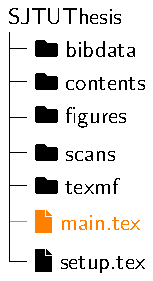
\includegraphics[page=1]{thesisdir}
    \end{column}
    \begin{column}{0.55\textwidth}
      \begin{codeblock}[firstnumber=3]{setup.tex}
\sjtusetup{
  info = {
    title    = {||上海交通大学学位论文 \LaTeX{} 模板示例文档},
    title*   = {A Sample for \LaTeX-based SJTU Thesis Template},
    author   = {||某\quad{}某},
    author* = {Mo Mo},
  },
  style = {
    header-logo-color = red,
  },
  name = {
    publications = {||攻读学位期间完成的论文},
  },
}
      \end{codeblock}
    \end{column}
  \end{columns}
\end{frame}

\begin{frame}[fragile]
  \frametitle{版权页}
  \framesubtitle{\texttt{\textbackslash{}copyrightpage}}
  \begin{columns}
    \begin{column}{0.45\textwidth}
      \only<1>{
        \includegraphics[page=9]{thesisdir}
      }
      \only<2>{
        \includegraphics[page=2]{thesisdir}
      }
      \only<3>{
        \begin{figure}[H]
          \framebox{\includegraphics[page=2,width=0.4\linewidth]{bachelor}}
          \caption{版权页}
        \end{figure}
      }
    \end{column}
    \begin{column}{0.55\textwidth}
      \begin{codeblock}[firstnumber=22]{main.tex}
|\highlightline<1>|% 原创性声明及使用授权书
|\highlightline<1>|\copyrightpage
|\highlightline<2>|% 插入外置原创性声明及使用授权书
|\highlightline<2>|% \copyrightpage[scans/sample-copyright-old.pdf]
      \end{codeblock}
      \only<1>{
        \cmd{copyrightpages} 可以用于插入版权页。
      }
      \only<2>{
        \cmd{copyrightpages} 也接受一个可选参数,用于直接使用扫描件。
      }
    \end{column}
  \end{columns}
\end{frame}

\begin{frame}[fragile]
  \frametitle{前置部分}
  \framesubtitle{\texttt{\textbackslash{}frontmatter}}
  \begin{columns}
    \begin{column}{0.45\textwidth}
      \only<1>{
        \includegraphics[page=9]{thesisdir}
      }
      \only<2>{
        \includegraphics[page=3]{thesisdir}
      }
      \only<3>{
        \begin{figure}[H]
          \begin{subfigure}{0.45\textwidth}
            \framebox{\includegraphics[page=3,width=\linewidth]{bachelor}}
            \caption{中文}
          \end{subfigure}\hfill
          \begin{subfigure}{0.45\textwidth}
            \framebox{\includegraphics[page=4,width=\linewidth]{bachelor}}
            \caption{英文}
          \end{subfigure}
          \caption{摘要}
        \end{figure}
      }
      \only<4>{
        \begin{figure}[H]
          \begin{subfigure}{0.30\linewidth}
            \centering
            \framebox{\includegraphics[page=5,width=0.6\linewidth]{bachelor}}
            \caption{目录}
          \end{subfigure}
          \begin{subfigure}{0.30\linewidth}
            \centering
            \framebox{\includegraphics[page=6,width=0.6\linewidth]{bachelor}}
            \caption{插图}
          \end{subfigure}

          \begin{subfigure}{0.30\linewidth}
            \centering
            \framebox{\includegraphics[page=7,width=0.6\linewidth]{bachelor}}
            \caption{表格}
          \end{subfigure}
          \begin{subfigure}{0.30\linewidth}
            \centering
            \framebox{\includegraphics[page=8,width=0.6\linewidth]{bachelor}}
            \caption{算法}
          \end{subfigure}
          \caption{索引}
        \end{figure}
      }
      \only<5>{
        \includegraphics[page=4]{thesisdir}
      }
      \only<6>{
        \begin{figure}[H]
          \framebox{\includegraphics[page=9,width=0.5\linewidth]{bachelor}}
          \caption{符号对照表}
        \end{figure}
      }
    \end{column}
    \begin{column}{0.55\textwidth}
      \begin{codeblock}[firstnumber=30]{main.tex}
|\highlightline<2-3>|% 摘要
|\highlightline<2-3>|\input{contents/abstract}

|\highlightline<4>|% 目录
|\highlightline<4>|\tableofcontents
|\highlightline<4>|% 插图索引
|\highlightline<4>|\listoffigures*
|\highlightline<4>|% 表格索引
|\highlightline<4>|\listoftables*
|\highlightline<4>|% 算法索引
|\highlightline<4>|\listofalgorithms*

|\highlightline<5-6>|% 符号对照表
|\highlightline<5-6>|\input{contents/nomenclature}
      \end{codeblock}
    \end{column}
  \end{columns}
\end{frame}

\begin{frame}[fragile]
  \frametitle{主体部分}
  \framesubtitle{\texttt{\textbackslash{}mainmatter}}
  \begin{columns}
    \begin{column}{0.45\textwidth}
      \only<1>{
        \includegraphics[page=5]{thesisdir}
      }
      \only<2>{
        \begin{figure}[H]
          \begin{subfigure}{0.30\linewidth}
            \centering
            \framebox{\includegraphics[page=11,width=0.6\linewidth]{bachelor}}
            \caption{简介}
          \end{subfigure}
          \begin{subfigure}{0.30\linewidth}
            \centering
            \framebox{\includegraphics[page=13,width=0.6\linewidth]{bachelor}}
            \caption{数学}
          \end{subfigure}

          \begin{subfigure}{0.30\linewidth}
            \centering
            \framebox{\includegraphics[page=16,width=0.6\linewidth]{bachelor}}
            \caption{浮动体}
          \end{subfigure}
          \begin{subfigure}{0.30\linewidth}
            \centering
            \framebox{\includegraphics[page=22,width=0.6\linewidth]{bachelor}}
            \caption{总结}
          \end{subfigure}
          \caption{主体部分}
        \end{figure}
      }
    \end{column}
    \begin{column}{0.55\textwidth}
      \begin{codeblock}[firstnumber=47]{main.tex}
|\highlightline|% 正文内容
|\highlightline|% !TeX root = ../../../latex-talk.tex

\section{是什么}

\begin{frame}
  \frametitle{\TeX{}}
  \begin{columns}[c]
    \begin{column}{0.7\textwidth}
      \begin{center}
        \rmfamily\Huge
        \highlight[structure]{\TeX{}}
      \end{center}
      \begin{center}
        \parbox{0.75\textwidth}{
          \TeX{} 是由斯坦福大学教授高德纳
          (Donald E.~Knuth)于 1977 年开始开发的排版引擎。目前仍在更新,最新版本号为 3.141592653 \link{https://tug.org/TUGboat/tb42-1/tb130knuth-tuneup21.pdf}。
        }
      \end{center}
    \end{column}
    \begin{column}{0.3\textwidth}
      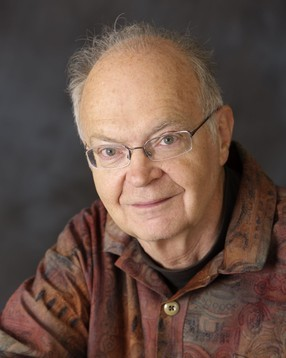
\includegraphics[width=.8\columnwidth]{support/images/Knuth.jpg}
    \end{column}
  \end{columns}
  \note{\emph{这一部分背景介绍大家可以了解一下,暂时跳过。}
  \LaTeX{} 这个词由两个部分组成,\hologo{La} 和 \TeX{}。那我们首先了解一下 \TeX{} 是什么。
  \TeX{} 是由斯坦福大学的教授高德纳于 1977 年开始开发的排版引擎,它已经有三十多年的历史了,
  目前仍在更新,版本号(3.141592653)将会趋近于 $\pi$ 的取值,高德纳最近还在给 \textsl{TUGBoat} 写稿子
  \link{https://tug.org/TUGboat/tb42-1/tb130knuth-tuneup21.pdf},
  关于 \TeX{} 今年又做了哪些改进。}
\end{frame}

\begin{frame}
  \frametitle{\LaTeX{}}
  \begin{columns}[c]
    \begin{column}{0.7\textwidth}
      \begin{center}
        \rmfamily\Huge
        \highlight[structure]{\LaTeX{}}
      \end{center}
      \begin{center}
        \parbox{0.75\textwidth}{
          \LaTeX{} 是最早在 1985 年由现就职于微软的 Leslie Lamport 开发的一种 \TeX{} \textbf{格式}\footnotemark,使用一些列宏和扩展宏包来简化 \TeX{} 的使用。现在由 \LaTeX{} Project 的成员维护。现在广泛使用的版本是 \LaTeXe{},最新的版本为 \LaTeX3(2020 年 10 月后默认内置)。
        }
      \end{center}
    \end{column}
    \begin{column}{0.3\textwidth}
      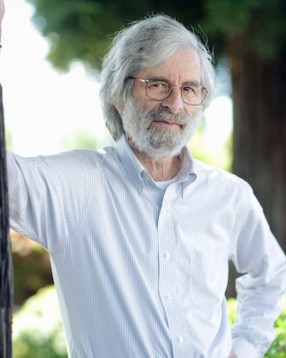
\includegraphics[width=.8\columnwidth]{support/images/Lamport.jpg}
    \end{column}
  \end{columns}
  \footnotetext{\hologo{ConTeXt} 也是一种 \TeX{} 格式 \link{https://www.contextgarden.net/}。}
  \note{\emph{这一部分的背景介绍大家可以了解一下,暂时跳过。}
  \LaTeX{} 是最早由现就职于微软的 Leslie Lamport 开发的一种 \TeX{} 格式(与其对标的是
  \hologo{ConTeXt}\link{https://www.contextgarden.net/}),主要也是为了简化 \TeX{} 的使用。
  现在主要由 \LaTeX{} 开发组维护,现在广泛使用的版本是 \LaTeXe{},最新的版本为 \LaTeX3,
  在 2020 年 10 月后默认内置,所以要尽可能使用较新的发行版,以充分发挥其功能。}
\end{frame}

\begin{frame}
  \frametitle{程序}
  \begin{columns}[c]
    \begin{column}{0.7\textwidth}
      \begin{center}
        \rmfamily\Huge
        \highlight[structure]{\hologo{pdfLaTeX}}
      \end{center}
      \begin{center}
        \parbox{0.7\textwidth}{
          \hologo{pdfLaTeX} 是为了编译一个 \LaTeX{} 文档而运行的程序。实际上底层在运行一个叫 \hologo{pdfTeX} 的引擎,并预装了对应的 \LaTeX{} \textbf{格式}。为了利用临时文件,可能就需要多次运行程序。
        }
      \end{center}
    \end{column}
    \begin{column}{0.3\textwidth}
      \begin{block}{}
        \ttfamily\small
        > \highlight{pdflatex} main.tex\\
        This is pdfTeX, Version 3.141592653-
        2.6-1.40.23 (MiKTeX 21.10)\\
        entering extended mode\\
        \highlight{LaTeX2e} <2021-11-15>\\
        \highlight{L3} programming layer <2021-11-22>
      \end{block}
    \end{column}
  \end{columns}
  \note{\hologo{pdfLaTeX} 是为了编译一个 \LaTeX{} 文档而运行的程序。}
\end{frame}

% \begin{frame}
%   \frametitle{引擎}
%   \begin{columns}[c]
%     \begin{column}{0.7\textwidth}
%       \begin{center}
%         \rmfamily\Huge
%         \highlight[structure!70]{pdf}\hologo{La}\highlight[structure!70]{\TeX{}}
%       \end{center}
%       \begin{center}
%         \parbox{0.7\textwidth}{
%           pdf\TeX{} 是编译 \TeX{} 文档(以 \texttt{.tex} 结尾)的\textbf{引擎}---可以理解 \TeX{} 指令的\textbf{程序}。
%         }
%       \end{center}
%     \end{column}
%     \begin{column}{0.3\textwidth}
%       \begin{block}{}
%         \ttfamily\small
%         > pdflatex main.tex\\
%         This is \highlight[structure!70]{pdfTeX}, Version 3.141592653-
%         2.6-1.40.23 (MiKTeX 21.10)
%         entering extended mode\\
%         LaTeX2e <2021-11-15>\\
%         L3 programming layer <2021-11-22>
%       \end{block}
%     \end{column}
%   \end{columns}
%   \note{实际上底层在运行一个叫 \hologo{pdfTeX} 的引擎,并预装了对应的 \LaTeX{} 格式。}
% \end{frame}

\begin{frame}[label={frame:engine}]
  \frametitle{程序}
  \begin{table}
    \caption{主流 \hologo{(La)TeX} 程序
    \footnote{(u)p\TeX{} 是日语最常用的引擎,生成 \texttt{.dvi},支持 Unicode。}\footnote{Ap\TeX{} \link{https://github.com/clerkma/ptex-ng} 具有底层 CJK 支持,内联 Ruby,Color Emoji。}}
    \footnotesize
    \begin{stampbox}
      \begin{tabular}{c>{\raggedright}*{3}{p{3.5cm}}}
        \alert{引擎}     & \hologo{pdfTeX}   & \hologo{XeTeX}   & \hologo{LuaTeX}   \\
        \alert{程序}     & \hologo{pdfLaTeX} & \hologo{XeLaTeX} & \hologo{LuaLaTeX} \\
        \alert{特点}     & 直接生成 PDF,支持 micro-typography  & 支持 Unicode、OpenType 与复杂文字编排 (CTL) & 支持 Unicode,内联 Lua,支持 OpenType \\
      \end{tabular}
    \end{stampbox}
  \end{table}

  \begin{center}
    \parbox{.9\textwidth}{
      \hologo{pdfLaTeX} 不支持 Unicode。为了排版中文,大部分情况下应当使用 \hologo{XeLaTeX},而 \hologo{LuaLaTeX} 速度相对较慢。\faWindows{} 可以在一些情况下使用 \hologo{pdfLaTeX}。
    }
  \end{center}
  \note{当然为了排版中文,已经不再推荐使用 \hologo{pdfLaTeX} 了,应该使用
  \hologo{XeLaTeX} 或者 \hologo{LuaLaTeX},当然后者的速度还是相对较慢,
  它们支持 Unicode 编码,并可以使用 OpenType 字体的全部功能。
  当然 \faWindows{} 平台下在某些追求速度的情况下,
  还是可以试着使用 \hologo{pdfLaTeX} 的。

  \hologo{LuaLaTeX} 理想情况下不慢,但是使用一些宏包后会破坏理想状态,
  也会因配置产生不同的结果,不同的操作系统在 I/O 速度上的不同也会导致不同的时间。

  \hologo{pdfLaTeX} 也支持,只不过需要先生成 tfm \TeX{} 字体度量文件,后续使用 \TeX{}
  自身的配置方法,只能使用 7 比特或 8 比特字体。}
\end{frame}

% \begin{frame}
%   \paragraph{\hologo{pdfLaTeX}} \TeX{} 和 \LaTeX{} 被广泛使用之前,它们只需内置支持欧洲语言即可。在 Unicode 出现之前,\LaTeX{} 提供了许多种\textbf{文件编码}来允许很多语言的文字以原生的方式输入,\hologo{pdfLaTeX} 也只需要使用 8 位文件编码和 8 位字体。
% \end{frame}


|\highlightline|\input{contents/math_and_citations}
|\highlightline|\input{contents/floats}
|\highlightline|% !TeX encoding = UTF-8
% !TeX root = ../latex-talk.tex

\section{总结}

\begin{frame}{常见 \LaTeX{} 困惑}
  \begin{itemize}
    \item \alert{编译不通过} 缺少必要宏包,命令拼写错误,括号未配对等
    \item \alert{表格图片乱跑} 非问题,\LaTeX{} 浮动定位算法 \link{https://liam.page/2017/04/30/floats-in-LaTeX-the-positioning-algorithm/}
    \item \alert{段落间距变大} 非问题,\LaTeX{} 排版算法
    \item \alert{参考文献} 推荐使用 \BibTeX{} 或者 Bib\LaTeX{}(视模板而定),也可以手写 \cmd{bibitem} \link{https://github.com/hushidong/biblatex-gb7714-2015}
  \end{itemize}
\end{frame}

\begin{frame}{系统学习}
  \begin{itemize}
      \item 包太雷 《\LaTeX{} Notes(第二版)》~(3小时)(lnotes2) \link{http://dralpha.altervista.org/zh/tech/lnotes2.pdf}
      \item Stefan Kottwitz 《LaTeX Cookbook》
      \item WikiBooks:英文 \link{https://en.wikibooks.org/wiki/LaTeX}、中文 \link{https://zh.wikibooks.org/wiki/LaTeX}
      \item 在线教程:OverLeaf 帮助文档 \link{https://www.overleaf.com/learn}
      \item 经典文档(亦可能比较过时)
        \begin{itemize}
          \item 仔细阅读《一份不太简短的~\LaTeXe{} 介绍》(lshort-zh-cn)~(1--2 天)
            \link{https://mirrors.sjtug.sjtu.edu.cn/CTAN/info/lshort/chinese/lshort-zh-cn.pdf}
          \item 粗略阅读《\LaTeXe{} 插图指南》~(2--3 小时)
        \end{itemize}
      \item 从~\SJTUThesis{} 示例文档入手
  \end{itemize}
\end{frame}

\begin{frame}{扩展阅读}
  \begin{itemize}
    \item 一份其实很短的 \LaTeX 入门文档 (Liam Huang) \link{https://liam.page/2014/09/08/latex-introduction/}
    \item 网站推荐:
      \begin{itemize}
        \item http://www.latexstudio.net/
        \item http://www.chinatex.org/
      \end{itemize}
    \item 知乎 \LaTeX{} 专栏(偏技术)\link{http://zhuanlan.zhihu.com/LaTeX}
    % \item \LaTeX{}杂谈(刘海洋)
    \item 《\LaTeX{}入门》(刘海洋)
    \item 现代 LaTeX 入门讲座(曾祥东)\link{https://github.com/stone-zeng/latex-talk/releases/tag/2019-04-18}
    \item “黑科技”:在 \LaTeX{} 中书写 Markdown 进行排版 \link{https://liam.page/2020/03/30/writing-manuscript-in-Markdown-and-typesetting-with-LaTeX/}
  \end{itemize}
\end{frame}


\begin{frame}[fragile]{利用文档}
  \begin{itemize}
    \item 常用文档
      \begin{itemize}
        \item \pkg{symbols}: 符号大全
        \item \pkg{Mathmode}: 数学参考
        \item \pkg{ctex}, \pkg{xeCJK}: 中文支持
        \item \pkg{texlive-zh}: \TL 安装与使用
        \item 所用宏包文档
      \end{itemize}
    \item 工具
      \begin{itemize}
        \item |tlmgr|: \TL 管理器
        \item |texdoc|: \TeX{} 文档查看器\\
          例如:|texdoc lshort-zh-cn|
        \item 在线文档 \TeX{}doc \link{http://texdoc.net/}
        \item TeX Studio 和 WinEdt 都支持在帮助里看文档
      \end{itemize}
  \end{itemize}
\end{frame}

\begin{frame}{一点人生的经验}
  \begin{itemize}
    \item 不要着急安装,先在 OverLeaf 上熟悉各类操作
    \item 不要过于相信网上的中文文档
      \begin{itemize}
        \item 简单鉴别方法: 排版的好看程度
      \end{itemize}
    \item 湿兄用U盘拷给你的的 \CTeX{} 套装一定是过时的,\SJTUThesis{} 八成是老版本的
    \item 如果你要处理中文
      \begin{itemize}
        \item 使用 \XeLaTeX{}, 使用 \XeLaTeX{}, 使用 \XeLaTeX{}
        \item 忘记 \pkg{CJK}, 忘记 \pkg{CJK}, 忘记 \pkg{CJK}
        \item 使用 \pkg{ctex} 宏包(2.0以上版本)(跟 \CTeX{} 套装仅仅是名字像)
      \end{itemize}
    \item 写一点,编译一次,减小排错搜索空间
  \end{itemize}
\end{frame}

\begin{frame}[fragile]
  \frametitle{Git版本管理}
  \begin{itemize}
    \item 版本管理的必要性
      \begin{itemize}
        \item 远离「初稿,第二稿……终稿,终稿(打死也不改了)」命名
        \item 方便与他人协同合作
      \end{itemize}
    \item 基本用法
      \begin{itemize}
        \item 跟踪更改:|git init|、|git add|、|git commit|
        \item 撤销与回滚:|git reset|、|git revert|
        \item 分支与高级用法:|git branch|、|git checkout|、|git rebase|
        \item 远端仓库操作:|git pull|、|git push|、|git fetch|
        \item 推荐用 VS Code 等进行可视化操作
        \item 参考链接:\link{https://git-scm.com/book/en/v2}
          \link{https://www.liaoxuefeng.com/wiki/0013739516305929606dd18361248578c67b8067c8c017b000}
      \end{itemize}
    \item 在线 Git 服务
      \begin{itemize}
        \item GitHub \href{https://github.com}{\faGithub}
        \item 上海交通大学源代码管理平台(基于 GitLab) \link{https://git.sjtu.edu.cn}
      \end{itemize}
  \end{itemize}
  \end{frame}

% 寻求帮助
\begin{frame}{求助}
  \begin{columns}[c]
    \begin{column}{.45\textwidth}
      \begin{itemize}
        \item BBS
          \begin{itemize}
            \item 水源社区 \link{https://dev.bbs.sjtu.edu.cn/}
            \item \sout{\CTeX 社区} (已关闭) \link{http://bbs.ctex.org/}
            \item 转移到 GitHub 的 \CTeX 社区 \link{https://github.com/CTeX-org/forum}
          \end{itemize}
        \item \TeX{} FAQ \link{https://www.texfaq.org/}
        \item \TeX{} StackExchange \link{https://tex.stackexchange.com/}
        \item Google, Bing, etc.
          \begin{itemize}
            \item 使用\textbf{英语}搜索
          \end{itemize}
      \end{itemize}
    \end{column}
    \begin{column}{.45\textwidth}
      
\includegraphics[width=\textwidth]{TFZsuperellipse-crop.pdf}
    \end{column}
  \end{columns}
\end{frame}

\begin{frame}{你也可以帮助}
  \begin{itemize}
    \item 错误反馈、改进建议:GitHub Issues \link{https://github.com/sjtug/SJTUThesis/issues}
    \item 出力维护:\LaTeX{} 宏包、模板编写,bug 修复
    \item 科普、答疑 
    \item \sout{来当主讲人}
  \end{itemize}
\end{frame}


%TC:ignore

% 参考文献
\printbibliography[heading=bibintoc]
      \end{codeblock}
    \end{column}
  \end{columns}
\end{frame}

\begin{frame}[fragile]
  \frametitle{参考文献}
  \begin{columns}
    \begin{column}{0.45\textwidth}
      \includegraphics[page=6]{thesisdir}
    \end{column}
    \begin{column}{0.55\textwidth}
      \begin{codeblock}[firstnumber=111,numbersep=2pt]{setup.tex}
% 使用 BibLaTeX 处理参考文献
%   biblatex-gb7714-2015 常用选项
%     gbnamefmt=lowercase     姓名大小写由输入信息确定
%     gbpub=false             禁用出版信息缺失处理
\usepackage[backend=biber,style=gb7714-2015]{biblatex}
% 文献表字体
% \renewcommand{\bibfont}{\zihao{-5}}
% 文献表条目间的间距
\setlength{\bibitemsep}{0pt}
|\highlightline|% 导入参考文献数据库
|\highlightline|\addbibresource{bibdata/thesis.bib}
      \end{codeblock}
    \end{column}
  \end{columns}
\end{frame}
